\documentclass[manual.tex]{subfiles}
\begin{document}

This section is meant as a guide to those who need to modify the SMAC code base for whatever reason.

\subsection{Design Overview}

The SMAC Application is broken up into three distinct projects as follows:

\begin{description}

\item[SMAC] Contains all of the logic that is specific to SMAC, (\eg{Validation, the SMAC algorithm, construction of SMAC Objects}). In essence it stitches together components of the Automatic Configurator Library. The sources are included in \texttt{smac-src.jar}.

\item[Algorithm Execution \& Abstraction Toolkit] Contains all of the primary abstractions/models used by SMAC (\eg{Object representations for Instances, Target Algorithm Configurations \& methods for executing algorithms,...}). 90\% of the code that SMAC uses lives in this library. It also contains code for converting the data from these abstractions into input needed to build the model. These are shipped with SMAC in the \texttt{aclib-src.jar} file. \textbf{Note}: Historically this was called "aclib", and in this version of SMAC internally the code still referred to it as aclib. The next version of SMAC will likely rename it.

\item[Random Forests] The Random Forest model code. The sources are included in \texttt{fastrf-src.jar}. 

\end{description}

The scope of this document governs only the first two projects. At the time of writing the \textbf{Algorithm Execution \& Abstraction Toolkit} has no published documentation, but if you e-mail the above a draft version is available.

\begin{itemize}

\item	The bulk of the code necessary to run SMAC lives in four classes \\ \texttt{AbstractAlgorithmFramework}, \\
 \texttt{SequentialModelBasedAlgorithmConfiguration}, \texttt{SMACBuilder} and finally, \\ \texttt{SMACExecutor}. 
\end{itemize}



\subsection{Class Overview}

The most important classes to SMAC are as follows:

\small
\begin{tabular}{ | c | p{10 cm} | }
\hline
\multicolumn{2}{|c|}{\textbf{Algorithm Execution \& Abstraction Toolkit}} \\
\hline
Name  & Description \\
\hline
\hline

\texttt{AbstractOptions}  & Base class for creating new options for SMAC. While not important
in and of itself, you will generally be implementing or modifying one of it's subtypes to implement options. \\
\hline

\texttt{AlgorithmRun} & Interface that represents the results of a target algorithm run. These are created by a \texttt{TargetAlgorithmEvaluator}. Outside of the \texttt{TargetAlgorithmEvaluator} these classes are generally immutable.\\
\hline

\texttt{AlgorithmExecutionConfig}  & Immutable object containing the information required to invoke a target algorithm. \\
\hline

\texttt{InstanceSeedGenerator}  & Interface that gets seeds for a \texttt{ProblemInstance}. These objects are constructed by \texttt{ProblemInstanceHelper}\\
\hline

\texttt{ModelBuilder}  & Interface whose implementations should result in a constructed model. \\
\hline

\texttt{OverallObjective}  & Aggregates many \texttt{RunObjective} values under some statistic ({\eg  mean}), to produce a value to be optimized. \\
\hline

\texttt{ParamConfiguration}  & Class that represents a specific setting of the target algorithm's parameters. This class also implements the \texttt{Map} interface, though does not support all the required operations. The ID associated with is object, is used only for logging and should not be used in the code. Finally although this class is not immutable the general life cycle is that the object is created, given specific values, and then never changed again. In future this may be augmented with the ability to prevent writes. These objects are always constructed via the \texttt{ParamConfigurationSpace}. \\
\hline

\texttt{ParamConfigurationSpace}  & (Almost immutable) class that represents the entire configuration space of a target algorithm. This class is constructed with the \textbf{Algorithm Parameter File} described in section \ref{sec:paramfile}. This class also contains the specifics of each parameter ({\eg domains, defaults, etc...}).  Currently the Random object used is the only portion that is mutable, and this will change in the future.\\
\hline

\texttt{ProblemInstance}  &  Immutable class that represents a specific problem instance, constructed by \texttt{ProblemInstanceHelper}.\\
\hline

\texttt{ProblemInstanceSeedPair}  &  Immutable class that represents a problem instance and seed. Decisions of which seed to use when scheduling a run are made in \texttt{RunHistory}.\\
\hline

\texttt{RunConfig}  & Immutable class that represents a problem instance seed pair, and configuration to execute.\\
\hline

\texttt{RunHistory}  & Interface that saves all the runs performed, and allows various queries against this information.\\
\hline
%%\end{tabular}

%%\small
%%\begin{tabular}{ | c | p{10 cm} | }
%%\hline
%%\multicolumn{2}{|c|}{\textbf{Automatic Configurator Library Classes}} \\
%%\hline
%%Name  & Description \\
%%\hline
%%\hline
\texttt{RunObjective}  & Converts an \texttt{AlgorithmRun} into a scalar value for optimization \\
\hline

\texttt{SanitizedModelData}  & Converts the run data into a format to use when building the model. Other things such as PCA, and other data filtering are done here. This interface and mechanism will likely be refactored in the future as it is brittle at the moment.\\
\hline

\texttt{SeedableRandomSingleton}  & A global random object whose existence is a convincing case that Singleton's are Anti-Patterns. This will, thankfully, go the way of the dodo bird at some point.\\
\hline

\texttt{StateFactory}  & Interface that constructs \texttt{StateSerializer} \& \texttt{StateDeserializer} to manage saving and restoring state respectively.\\
\hline

\texttt{TargetAlgorithmEvaluator}  & Interface whose implementations should be able to run the algorithm (\ie{ Implementations should convert \texttt{RunConfig} objects to \texttt{AlgorithmRun} objects}). See section \ref{sec:target-algorithm-evaluators}  for more information. \\
\hline
\end{tabular}

\vspace{25pt}

\begin{tabular} { | c | p {6 cm} | }
\hline
\multicolumn{2}{|c|}{\textbf{SMAC Library Classes}} \\
\hline
Name  & Description \\
\hline
\hline



\texttt{AbstractAlgorithmFramework } & \emph{Non-abstract} class that provides a default Automatic Configurator (ROAR)\\
\hline

\texttt{SequentialModelBasedAlgorithmConfiguration} & Class that subtypes \texttt{AbstractAlgorithmFramework} and implements the methods required for SMAC \\

\hline 
\texttt{SMACExecutor} & Parses command line options and creates some of the objects SMAC needs to execute (SMAC entrypoint)\\
\hline

\texttt{SMACBuilder} & Takes the options parsed by SMACExecutor or some other utility, and builds everything necessary to create an instance of \texttt{AbstractAlgorithmFramework}. If you want to plug smac into your application, you generally want to mimic what SMACExecutor does to invoke SMACBuilder.\\
\hline


\hline
\texttt{Validator} & Performs Validation of selected configurations\\
\hline

\texttt{ValidatorExecutor} &  Entry point to stand alone validation utility\\
\hline

\end{tabular}

\normalsize

\subsection{SMAC Sequence Diagram}

\begin{figure}[h]
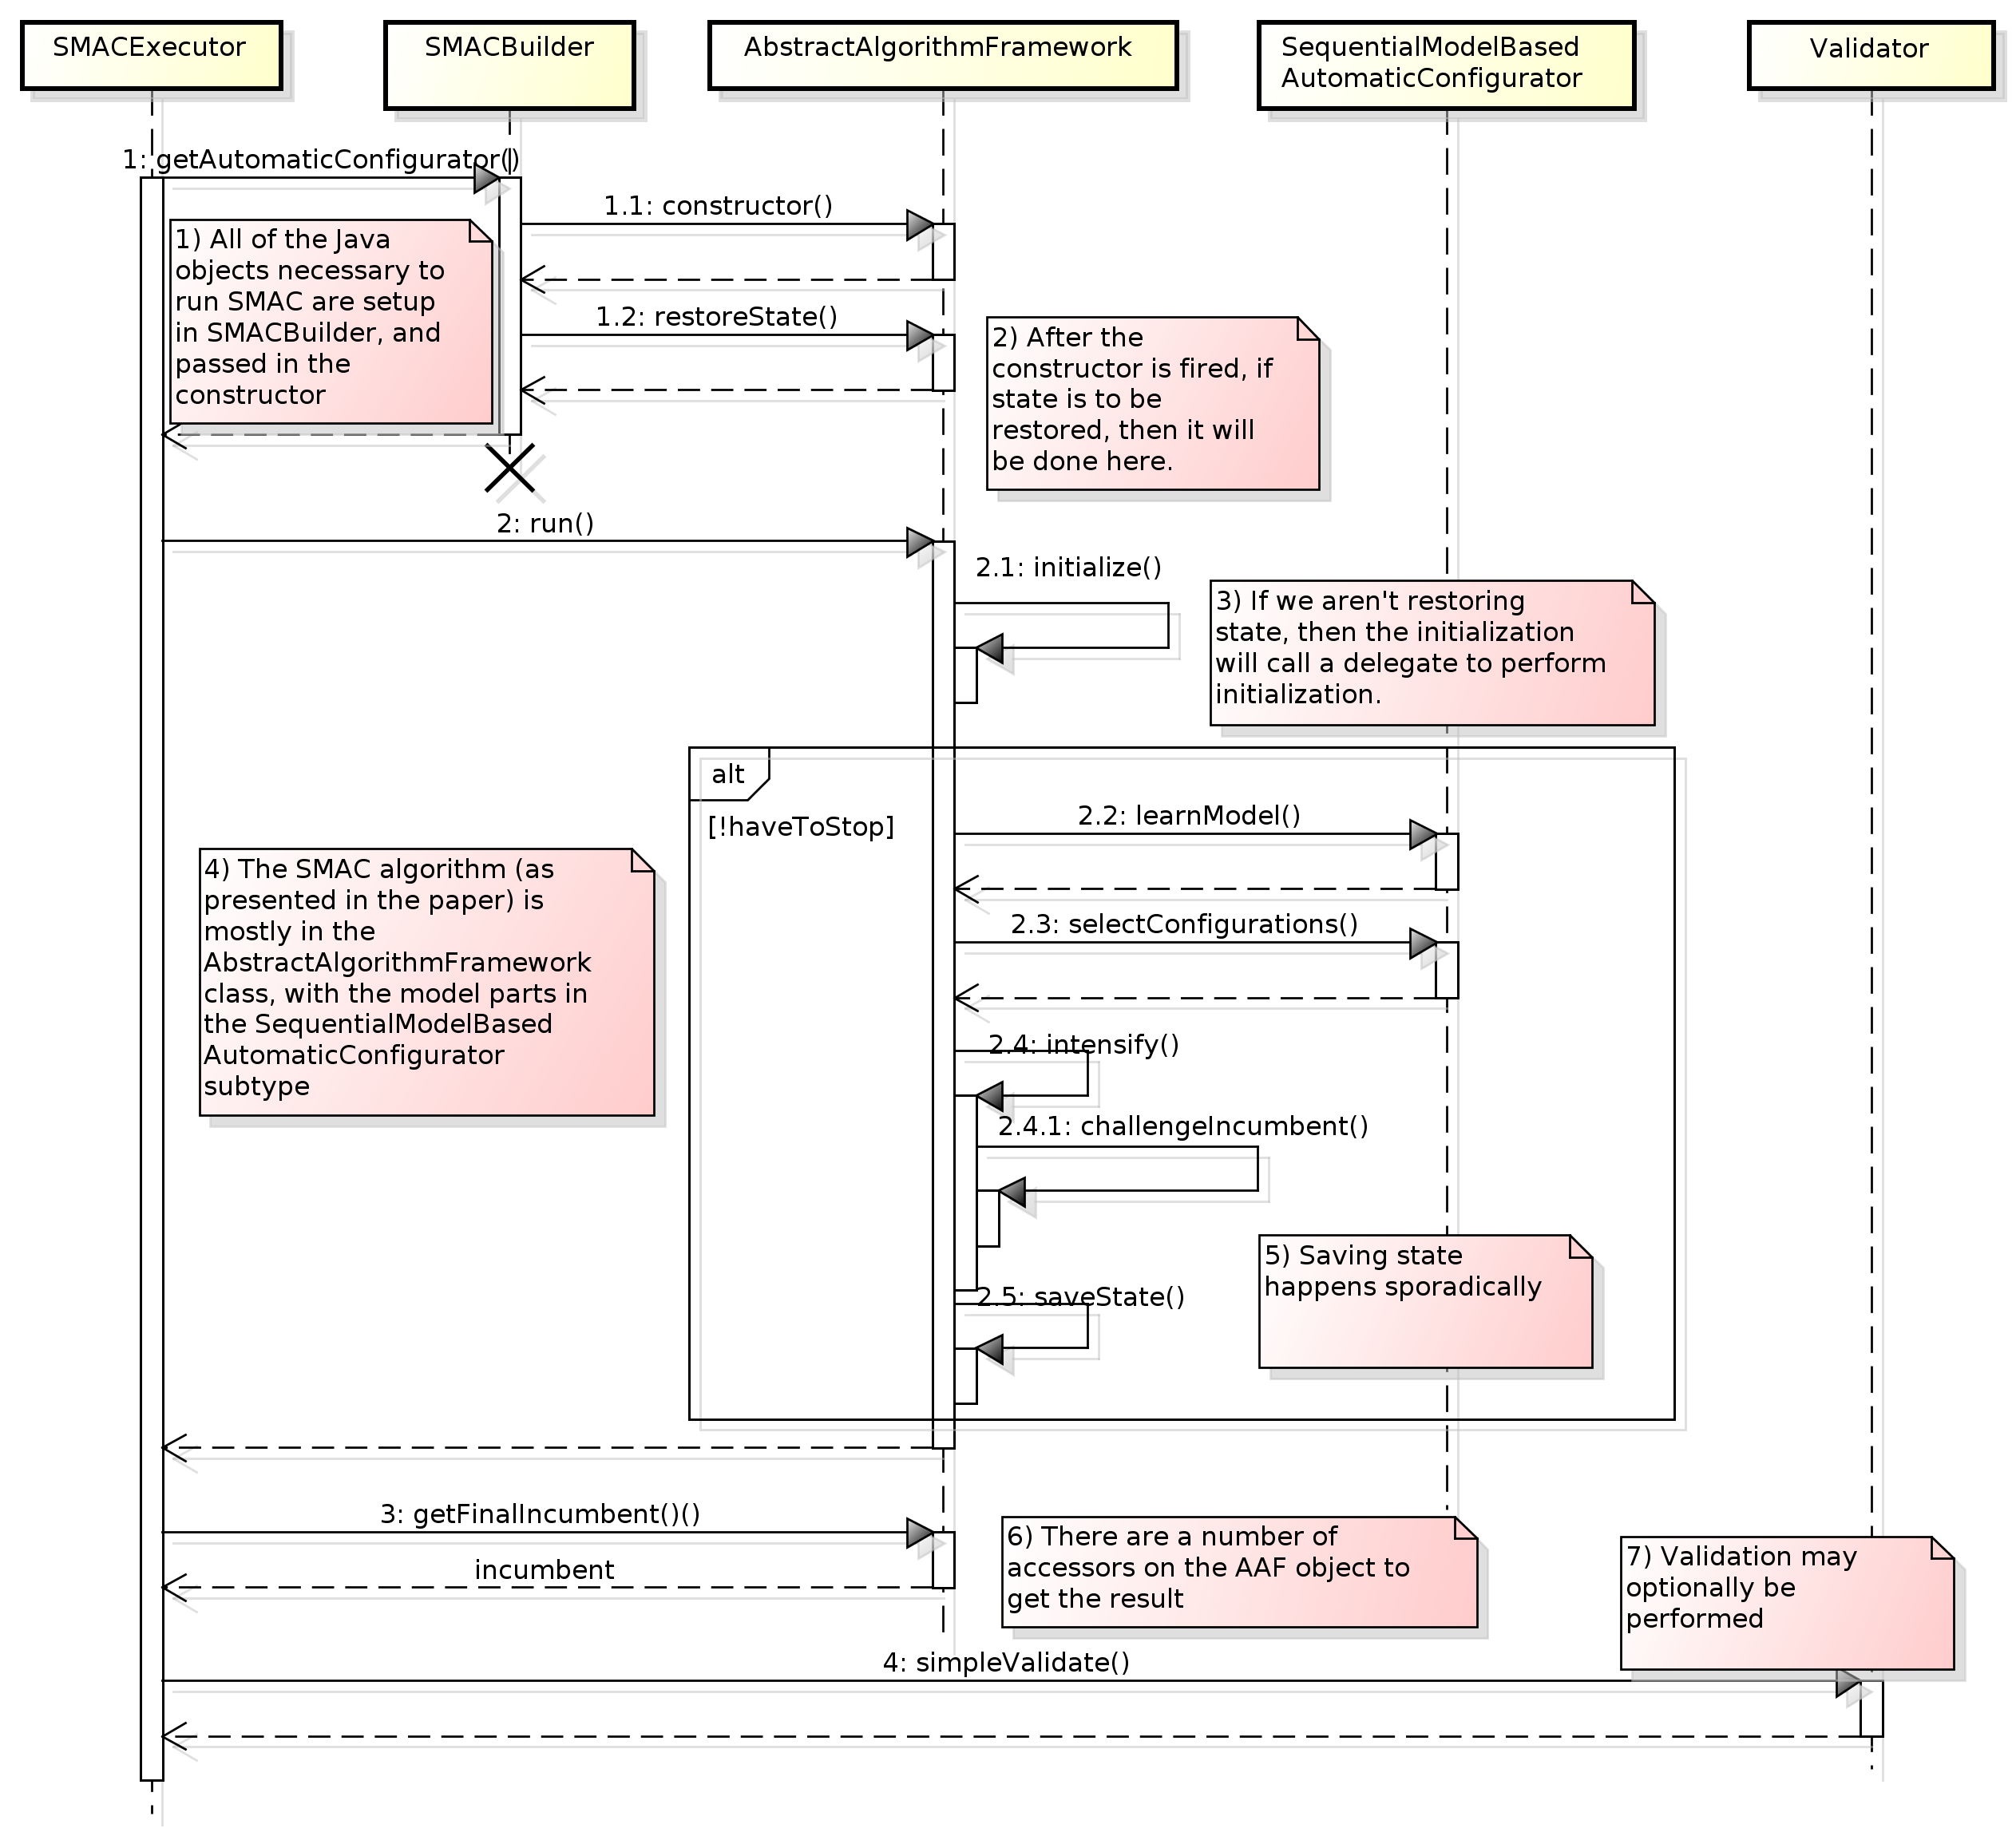
\includegraphics[height=18cm,angle=0, trim=2.5cm 0cm 0cm 0cm clip=true]{sequence.png} 
\caption{Sequence diagram detailing the execution of a standard SMAC run}
\label{sequence}
\end{figure}

See Figure \ref{sequence} on page \pageref{sequence} for a sequence diagram relating the 5 main classes.

\subsection{Algorithm Execution \& Abstraction Toolkit}

At some future point a better guide will be available, in the interim please e-mail the authors above for a draft.

\subsection{Running SMAC in Eclipse}

Depending on what you would like to do it might be better to ask for git repository access, which contains ant build scripts and an existing eclipse project. The following procedure however will get you a working installation in eclipse. 

\textbf{NOTE:} This guide is pretty straight forward except for step 10 \& 11, so if you are comfortable with Eclipse you should just skip to those steps.

To start the smac project project in eclipse do the following:
\begin{enumerate}

\item Create a new project in Eclipse, ensure that the JDK is 1.7 or higher.

\item Create a new source folder: \texttt{aeatk}

\item Create a new source folder: \texttt{smac}

\item Create a new source folder: \texttt{fastrf}

\item Create a new folder: \texttt{lib}

\item Copy all the jar files from the \texttt{lib} folder of the SMAC release into the lib folder of the eclipse project, except for \texttt{smac.jar}, \texttt{smac-src.jar}, \texttt{aeatk.jar}, \texttt{aeatk-src.jar}, \texttt{fastrf.jar} and \texttt{fastrf-src.jar}.

\item Unzip the \texttt{smac-src.jar} into the smac source folder

\item Unzip the \texttt{aeatk-src.jar} into the aeatk source folder

\item Unzip the \texttt{fastrf-src.jar} into the fastrf source folder.

\item Right click on the project and go to Properties $\rightarrow$ Java Compiler $\rightarrow$ Annotation Processing and check the \emph{Enable project specific settings} and \emph{Enable annotation processing}.

\item Then in the project properties navigate to Java Compiler $\rightarrow$ Annotation Processing $\rightarrow$ Factory Path and hit \emph{Add Jars} then select \texttt{lib/spi-0.2.4.jar} and hit OK.

The entry point of any application can be retrieved from the shell script folder, for instance by opening the smac file we can see that the entry point is: \texttt{ca.ubc.cs.beta.smac.executors.SMACExecutor} and smac-validate is : \texttt{ca.ubc.cs.beta.smac.executors.ValidatorExecutor}

Many of the helper utilities are contained in the \texttt{ca.ubc.cs.beta.aeatk.example.} subpackages.

\end{enumerate}

\textbf{NOTE:} If you try and run existing scenarios packaged with SMAC they contain paths relative to the root of the smac dir. So in your \emph{Run Configuration} you should set the \emph{Working Directory} to the root of some smac release to run it as you would on the command line.


If when running SMAC you see either of the following errors:

\textcolor{red}{
WARNING: I could not find ANY Target Algorithm Evaluators on the classpath.\\
 If you made this JAR (or setup the classpath) yourself chances are you did not setup SPI correctly.
 You must ensure that in the JAR (or on the classpath) there is a \\
  META-INF/services/ca.ubc.cs.beta.aeatk.targetalgorithmevaluator.TargetAlgorithmEvaluatorFactory file \\
 In this file should list every implementation of that interface 
}
\vspace{10pt}

This means you did not follow steps 10 \& 11 properly.

%
%
%{\Large\textbf{\textsc{\textcolor{red}{Warning:}}}  The Target Algorithm Evaluator API has changed a bit since this section was written, you are encouraged to look in the code for an example of how it now works. Much of this is still relevant, and this section will be fixed for v2.08.00, but for v2.06.00 it will contain some inaccuracies.}\\
%
%\label{sec:target-algorithm-evaluators}
%
%The \textbf{Target Algorithm Evaluator} subsystem is the part of the code you will be modifying if you would like to change how target algorithms are run. On the next page is a UML class diagram showing most of how this part of the code works.
%
%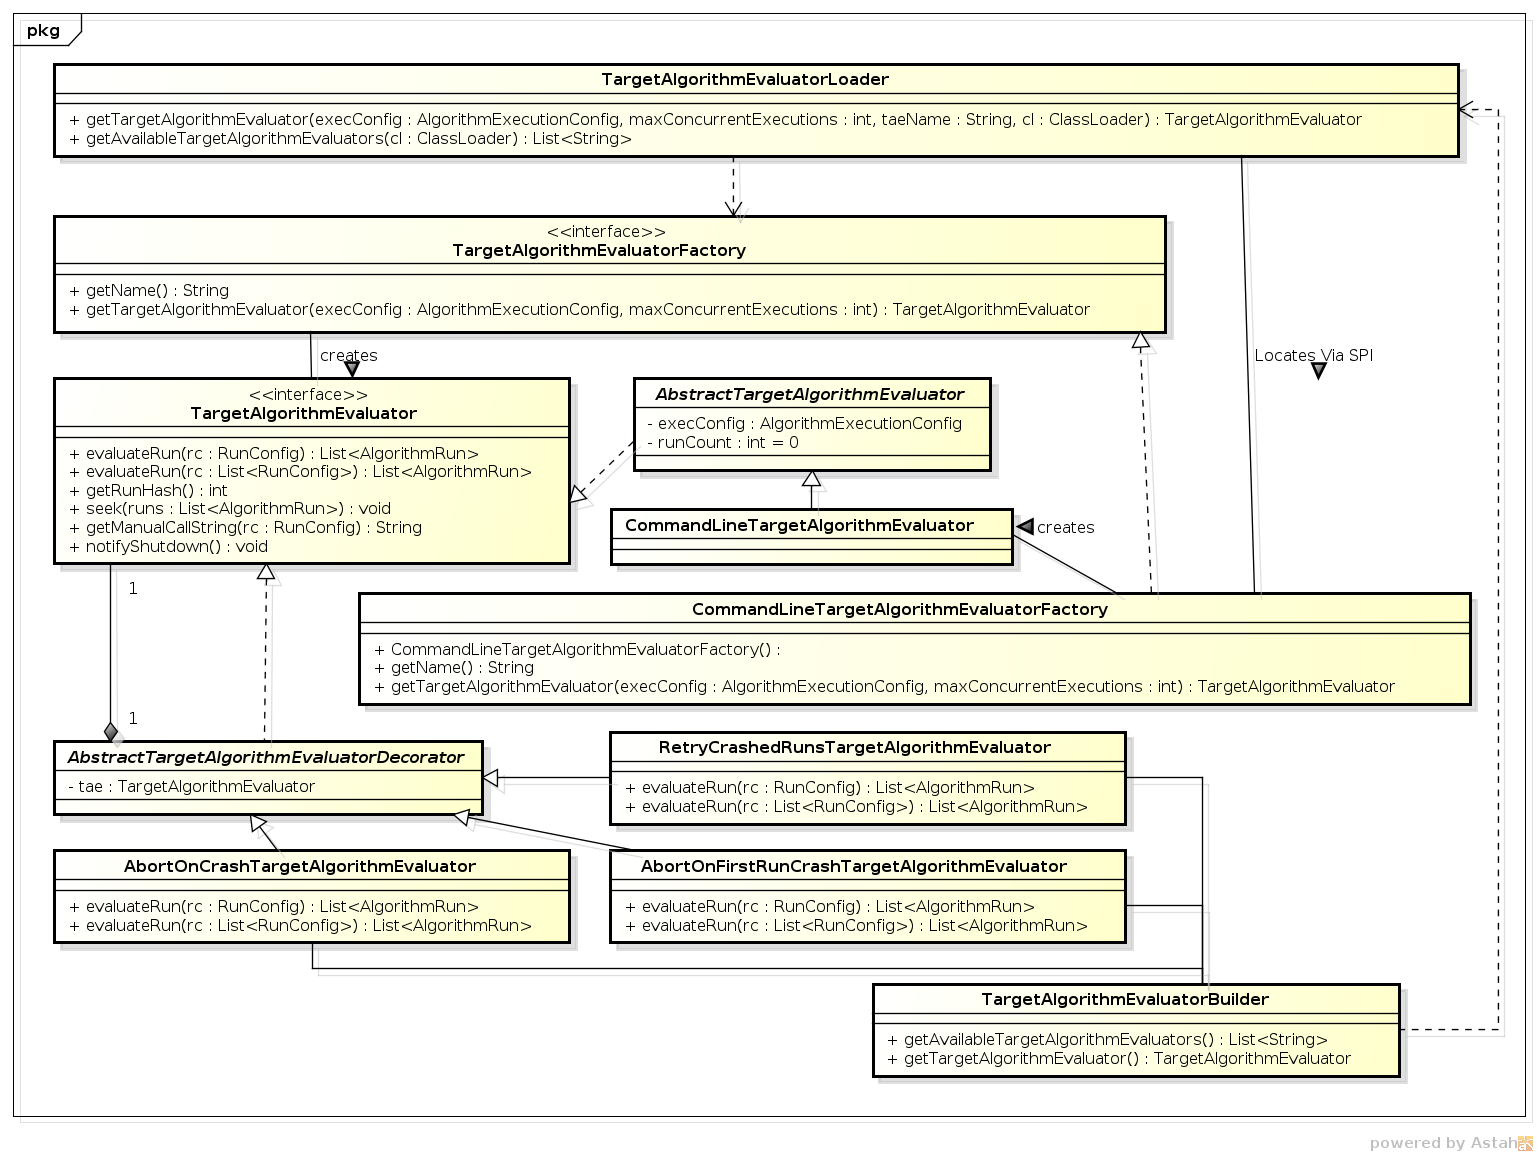
\includegraphics[height=18cm,angle=270, trim=4cm 0cm 0cm 0cm clip=true]{tae.png} 
%
%\vspace{15pt}
%Once constructed, the \texttt{TargetAlgorithmEvaluator} interface is simple, it simply needs to return a new \texttt{AlgorithmRun} object, for each \texttt{RunConfig} object passed as input, and in the same order, via the \texttt{TargetAlgorithmEvaluator.evaluateRun()} method. The construction of these objects is where the complexity lies and so here is a run through of the construction.
%
%\begin{enumerate}
%
%\item When the code starts up, SMAC requests a specific Target Algorithm Evaluator (using some globally unique String as a key), from \texttt{TargetAlgorithmEvaluatorBuilder.getTargetAlgorithmEvaluator()} 
%
%\item This invokes the similarly named method in \texttt{TargetAlgorithmEvaluatorLoader}, which uses SPI (see \ref{sec:plugin-versioning} for more information on SPI) to find the \texttt{TargetAlgorithmEvaluatorFactory} whose \texttt{getName()} method returns the matching string. The name \textsc{must not}  have any white space. For reference, the \\ \texttt{CommandLineTargetAlgoirthmEvaluatorFactory} returns \texttt{CLI}.
%
%\item When an match is found, a no argument constructor (in the diagram this is shown under the \texttt{CommandLineTargetAlgorithmEvaluatorFactory} class) is invoked. 
%
%\item Next the \texttt{getTargetAlgorithmEvaluator()} method is invoked which in the above diagram would return a \texttt{CommandLineTargetAlgorithmEvaluator}
%
%\item With this new instance in hand, the \texttt{TargetAlgorithmEvaluatorBuilder} then wraps this object with various decorators (\eg{RetryCrashedRunTargetAlgorithmEvaluator}) depending on the options supplied (not-shown).
%
%\end{enumerate}
%
%The use of SPI allows new implementations to be created without modifying the existing SMAC code, and requires less mantinence to update to newer versions of SMAC. Unfortunately at the time of writing there are two limitations to keep in mind with this approach.
%
%\begin{enumerate}
%
%\item You cannot supply options to the user to configure your \texttt{TargetAlgorithmEvaluator}.
%
%\item You cannot use this method to add new decorators. 
%
%\end{enumerate}
%
%Neither of these seems significant at the current time. If a new decorator is needed, you can hard code the base implementation and return a wrapped instance of it (\ie{Create a new \texttt{TargetAlgorithmEvaluatorFactory} that returns a wrapped instance of an existing \texttt{TargetAlgorithmEvaluator}}). Configuration of the \texttt{TargetAlgorithmEvaluator} can be done via files at this point.
%
%When using the SPI approach you are strongly encouraged to also implement \textbf{Plugin Versioning}; see Section \ref{sec:plugin-versioning}.
%
%
%\subsection{Plugin Versioning}
%\label{sec:plugin-versioning}
%
%Any plug-ins or changes to SMAC should contain an implementation of \texttt{VersionInfo}, and 
%the implementor should be labelled as a provider of \texttt{VersionInfo} via SPI \footnote{SPI is the Service Provider Interface, see SPI on Wikipedia (\url{http://en.wikipedia.org/wiki/Service_provider_interface}) as well as this utility which simplifies the process drastically (\url{http://code.google.com/p/spi/})}.
%
%In essence this interface simply has two getter methods \texttt{getProductName()} and \texttt{getVersion()}. If everything is done correctly when SMAC starts up you should 
%see the product name and version printed in the logs.
%
%\textbf{Example:}
%\small
%\begin{verbatim}
%[INFO ] Version of Automatic Configurator Library is v2.06.00-development-583 (2e12acc92f41) 
%[INFO ] Version of Random Forest Library is v1.05.01-development-95 (4a8077e95b21) 
%[INFO ] Version of SMAC is v2.06.00b-development-561 (abb03ff41e82) 
%\end{verbatim}
%\normalsize 
%	This can make debugging and managing reproducibility much easier. Most projects include the first 12 characters of the git commit hash to make it easy to find that commit.
%	
%	
%\subsection{Run Hash Codes}
%
%A Run Hash Code is a sequence of hashes that represent which runs
%were scheduled by SMAC. 
%When calling SMAC using\\
%\texttt{./smac~-{}-scenarioFile~<file>~-{}-runHashCodeFile~<logfile>},\\
%SMAC logs all Run Hash Codes to $<$logfile$>$.
%This option allows reading of that log file for subsequent runs to ensure that the exact same set of runs is scheduled. This is primarily of use for developers.

	
\end{document}